\documentclass{article}
\usepackage{geometry}
\usepackage{graphicx}
\usepackage{amsmath}
\usepackage{algorithm}
\usepackage{algpseudocode}
\usepackage{makeidx}

\makeindex

\geometry{
a4paper,
top=10mm,
bottom=15mm,
left=10mm,
right=10mm,	
}

\begin{document}

\pagenumbering{gobble}
\newgeometry{
top=30mm,
bottom=50mm,
left=20mm,
right=20mm,
}

\begin{center}

\textbf{\Huge Biased Die} \\
\vspace{50pt}
{\large Assignment 7 } \\
\textbf{\large CS251: Computer Laboratory} \\
\vspace{100pt}

\textbf{\large Jayant Agrawal} \\
(14282)
\vspace{30pt}

INSTRUCTOR \\
\textbf{Prof. Arnab Bhattacharya}
\vspace{100pt}


\includegraphics[width=0.3\columnwidth]{logo.jpg}\\
\textbf{\large Department of Comuter Science and Engineering \\
INDIAN INSTITUTE OF TECHNOLOGY KANPUR \\
KANPUR 208016, INDIA \\ } 
\vspace{20pt}
March 2016

\end{center}

\restoregeometry
\newpage
\pagenumbering{roman}
\tableofcontents
\addcontentsline{toc}{section}{\listfigurename}
\addcontentsline{toc}{section}{\listtablename}
\listoffigures
\listoftables


\newpage
\pagenumbering{arabic}

\section{Introduction}
A cubical dice has 6 faces, numbered 1,2,3,4,5,6. A fair dice on random throw can give any of the face with equal probability. Figure \ref{fig:dice} shows the picture of a dice.
\begin{figure}[h!]
\begin{center}
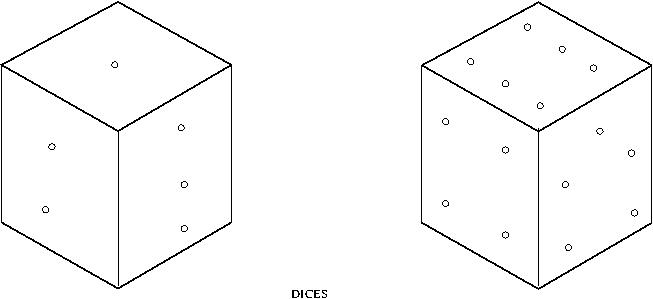
\includegraphics[width=0.7\columnwidth]{script3.jpeg}
\label{fig:dice}
\caption{Dice: Different Orientation}
\end{center}
\end{figure}


\section{Expectation}
\index{Expectation} Expectation of a random variable is the long-run average value of repetitions of the experiment. 
Let X be any random variable. Let the sample space be U.
$$U = {a_1,a_2,......,a_n}$$
Let P be the set of probabilities.

$$ P={p_1,p_2,......,p_n}$$

Then expexted value of the \index{random variable}random variable X is
$$E(X) = \sum_{i=1}^{n}X(a_i) \times p_i$$

For a dice 
U=\{1,2,3,4,5,6\}
and $$ \sum_{i=1}^{6}(P_i)=1$$

\section{The Experiment}

\begin{figure*}[!t]
        \begin{center}
                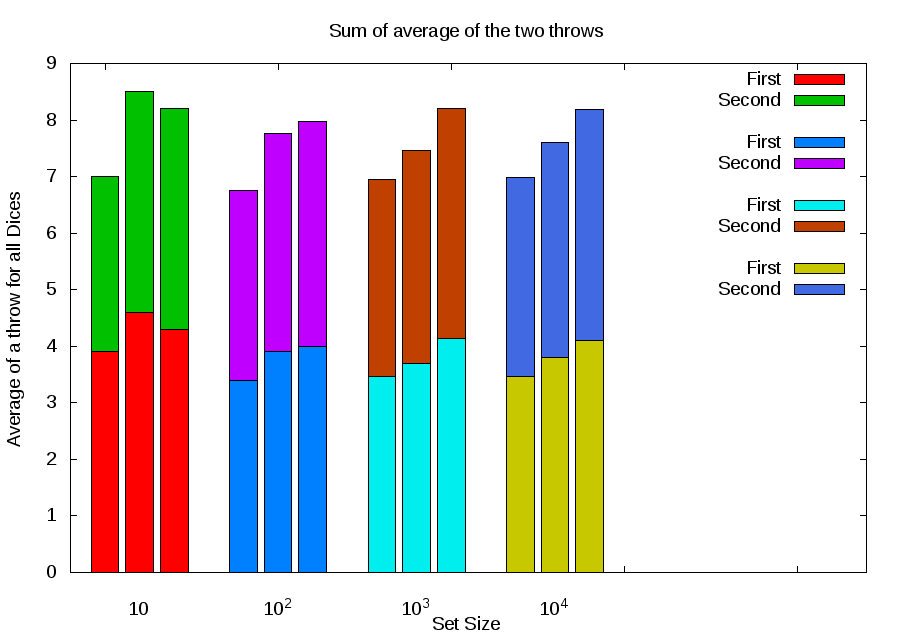
\includegraphics[width=0.8\columnwidth]{histforall.png}
        \end{center}
	\caption{Histogram}
	\label{fig:Sum of averages for dice 1,2,3 for different set sizes}
\end{figure*}

\begin{table}[h]
    \centering
    \begin{tabular}{||c|c|c|c|c|c||}
 \hline       
(1 1) & (1 2)  & (1 3) & (1 4) & (1 5) & (1 6) \\
\hline
(2 1) & (2 2) & (2 3) & (2 4) & (2 5) & (2 6) \\
\hline
(3 1) & (3 2) & (3 3) & (3 4) & (3 5) & (3 6) \\
\hline
(4 1) & (4 2) & (4 3) & (4 4) & (4 5) & (4 6) \\
\hline
(5 1) & (5 2) & (5 3) & (5 4) & (5 5) & (5 6) \\
\hline
(6 1) & (6 2) & (6 3) & (6 4) & (6 5) & (6 6) \\
\hline 
    \end{tabular}
    \caption{Sample space for throwing a pair of die}
    \label{table:one}
\end{table}


\begin{table}[h]
    \centering
    \begin{tabular}{||c|c|c|c|c|c|c||}
\hline 
Possible outcome & 1 & 2 & 3 & 4 & 5 & 6 \\
\hline
Probabilties for die 1 & 1/6 & 1/6 & 1/6 & 1/6 & 1/6 & 1/6 \\
\hline
Probabilities for die 2 & 17/120 & 17/120 & 17/120 & 17/120 & 13/60 & 13/60 \\
\hline
Probabilities for die 3 & 7/60 & 7/60 & 7/60 & 7/60 & 4/15 & 4/15 \\
\hline
     \end{tabular}
     \caption{Probability distribution}
     \label{table:two}
\end{table}


\section{Histogram}
From Table \ref{table:two}, one can find the expected value of sums for die 1, die 2 and die 3.\\

\begin{itemize}
\item Expected value of sum for die1 = 7
\item Expected value of sum for die2 = 7.6
\item Expected value of sum for die3 = 8.2
\end{itemize}

For dice 1 every outcome is equally likely and hence expectation is the average of all possible outcomes.
While for die 2 and 3 the probability of higher outcome(5,6) as output is higher and hence expectation for them is higher.
In case of die 3 their is more baising so expectation for die 3 is more than that of die 2.

\section{Conclusion}
The expected value is greatest in die 3 followed by die 2 and least in die 1.

\addcontentsline{toc}{section}{References}
\newpage
\addcontentsline{toc}{section}{Index}
\printindex
\end{document}
